\chapter{Introduction}
\label{chapter:body}
\thispagestyle{myheadings}
\setcounter{tocdepth}{1}
% set this to the location of the figures for this chapter. it may
% also want to be ../Figures/2_Body/ or something. make sure that
% it has a trailing directory separator (i.e., '/')!
\graphicspath{{1_Intro/Figures/}}

Incoherent scatter radar (ISR), like all scientific instruments, is a testament to humankind's desire to understand the world around it. This even more so because they are generally very large and complicated systems that use substantial amounts of power, in the range of megawatts. These systems are able to probe Earths ionosphere and unlike other ground based measures this modality can give direct measurements of various plasma parameters including electron density ($N_e$), electron temperature ($T_e$), ion temperature ($T_i$) and ion velocity ($V_i$). ISRs has been in use since the 1950s \cite{gordon58} and these systems have evolved over time from only being able to measure parameters along a single line of site to recently having the ability to be used as full 3-D sensors. The goal of this dissertation is to present a framework to analyze and improve the quality of the data that comes from modern �ISR systems. This framework can help researchers improve their experiments and better understand the data products from ISR.

Until recently these systems were constructed using single, mechanically steered antennas. Because of this the rate that the look angle can change is limited by the mechanical speed of the \jcom{doesn't sound right}{antenna pointing mechanism.} The newest generation of ISR systems are now taking advantage of electronically scanning phased array (ESPA), which allow for a near instantaneous change in the radar look direction. This thesis will mainly focus on systems that are equipped with ESPA antennas, as they are the impeddous for this work. Still many if not all of these ideas contained within can still be used by researchers using systems using single mechanically steered antennas or by individuals using the ESPA equipped ISR systems that using it to observe phenomena along just the range dimension.




 
\section{Purpose}
Some of the basics of ISR will be introduced in the following section. This along with a short discussion of the ionosphere and some of the phenomena that researchers use ISR to observe. Following this will be a short introduction to some of the basic precepts behind inverse theory as used by engineers and scientists to analyze and improve the output of sensors.

\subsection{Incoherent Scatter Radar}

In order to produce plasma parameter measurements ISR systems radiate electromagnetic energy and monitor the reflected signal from free electrons in the ionosphere, or observe from other radiation sources in bistatic operation. This scatter has a specific spectral distribution from which is driven by the values of the temperatures, densities and bulk flow of the plasma in the ionosphere. As such the two main steps in processing is the estimation of a power spectrum or autocorrelation function (ACF) and then fitting that to a physics based model at each point in time and space that the radar samples. 

As stated previously ESPA antennas can create three dimensional reconstructions of plasma parameters. Examples of these new systems include The Advance Modular Incoherent Scatter Radars (AMISR), that have been developed and placed in Poker Flat Alaska and in Resolute Bay Canada. These systems have already started to give unprecedented views in the ionosphere and upper atmosphere. Currently EISCAT-3D is being developed as well and is expect do give even greater views due to the multi-static set up.


\subsection{Ionosphere and Phenomena}
The ionosphere is the area of partially ionized gas, or plasma, surrounding the earth and in a way is like an interface between the earth and outer space \cite{kellybook}. The dynamics of this system are governed by kinetic, fluid and Maxwells equations coupled together \cite{schunk2004ionospheres}. This complicated menagerie of equations allows for the creation of a cornucopia of different phenomena at any number of spatio-temporial scales.

%In order to understand the behavior of the plasma in the ionosphere one needs to use electromagnetic theory governed by Maxwells Equations seen in Equations \ref{eqn:max1} and \ref{eqn:max2},

%\begin{eqnarray}
%\label{eqn:max1}
%\nabla \cdot \vec{E} = \frac{\rho}{\epsilon_0}\  &&\nabla  \cdot \vec{B} = 0 \nonumber \\
%\nabla  \times \vec{E} = - \frac{\partial B}{\partial t} && \nabla  \times \vec{B} = \mu_{0}\vec{J} +
%\mu_{0}\epsilon_{0}\frac{\partial E}{\partial t}
%\end{eqnarray}
%
%\begin{equation}
%\label{eqn:max2}
%\frac{\partial \rho}{\partial t}+\nabla \cdot \vec{J} = 0
%\end{equation}
% 
%\noindent where $\rho$ is the charge density, $\vec{E}$ is the electric field, $\vec{B}$ is the magnetic field, $\vec{J}$ is the current density, $\mu_0$ is the vacuum permeability and $\epsilon_0$ is the vacuum permittivity. 
%
%In order to close the system of equations often assumptions about the charge density and current density are needed \cite{varnytalk2016}. In the ionosphere though $\vec{J}$ is linked to the electric and magnetic fields, $\vec{E}$ and $\vec{B}$, which are dependent on the particle motion. In the ionosphere these particles move as gas, so to close these systems of equations require the use of fluid and/or kinetic theory depending on what sort of assumptions can be made for the problem.

When studying the ionosphere at times it helpful to look at a specific region. The high latitude ionosphere, which is the region close to the earth's magnetic poles, is of special interest due to the number of different phenomena that occur in this region. These phenomena include but are not limited to aurora borealis, polar cap plasma patches and particle precipitation events. 

The following is a listing of examples various types of high latitude ionosphere events grouped by specific behavior that is of interest the ISR sampling problem.

\begin{figure}[!t]
\centering
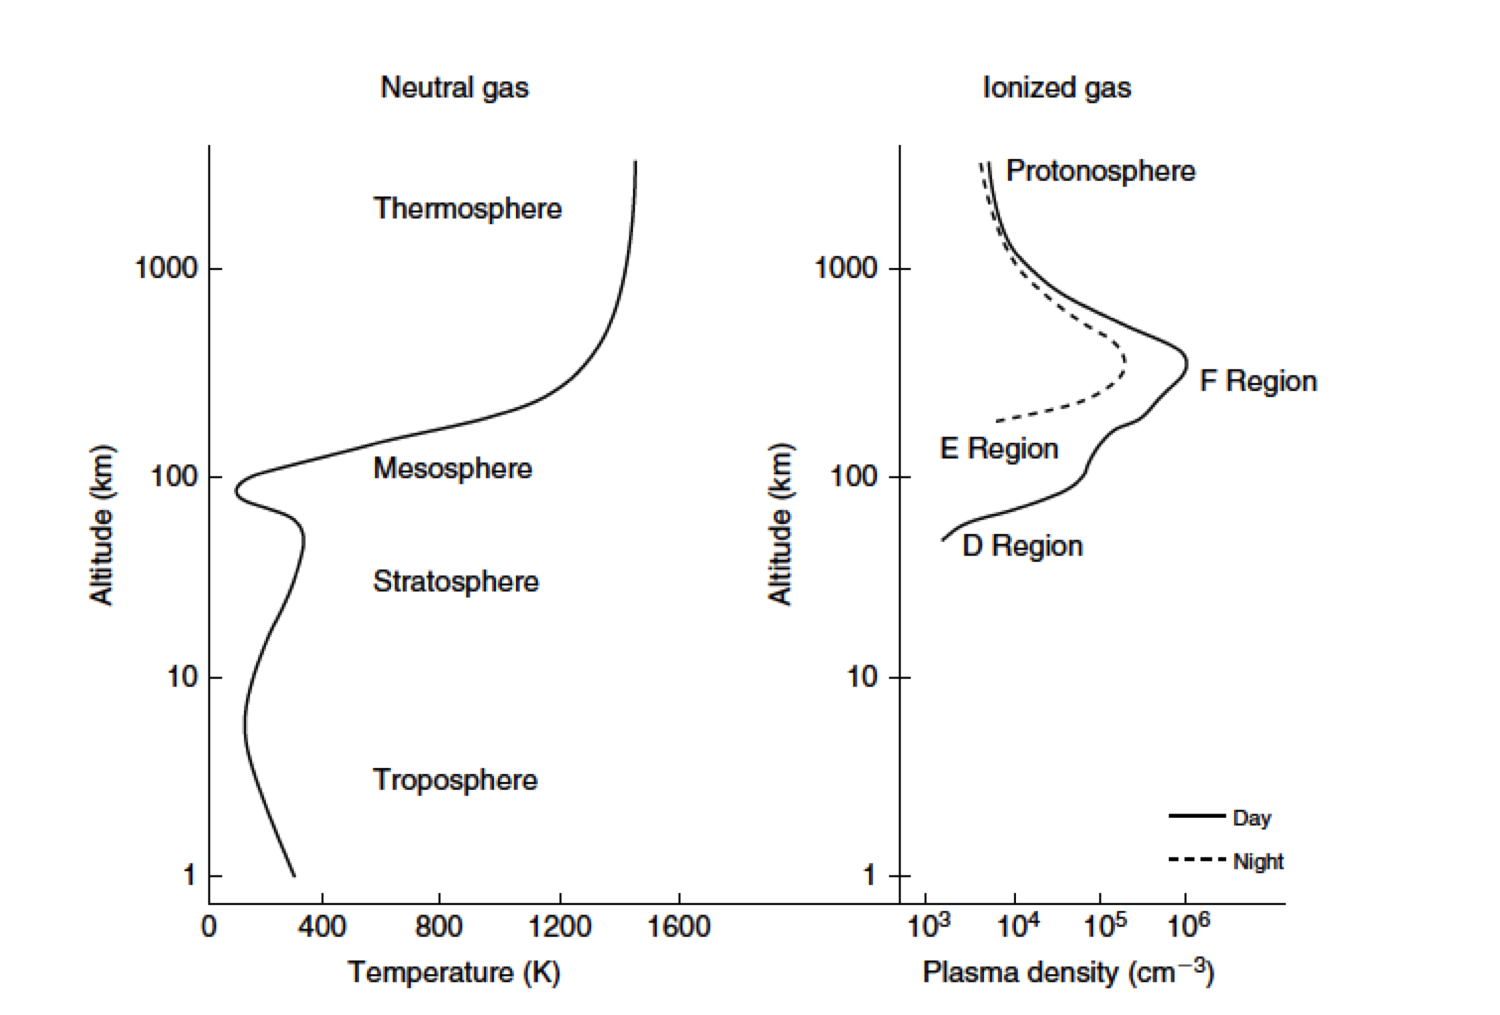
\includegraphics[width=5in]{altvsparams}
% where an .eps filename suffix will be assumed under latex, 
% and a .pdf suffix will be assumed for pdflatex; or what has been declared
% via \DeclareGraphicsExtensions.
\caption{Example profiles of neutral temperature and plasma density from \cite{kellybook}}
\label{fig:singlefilt}
\end{figure}
%These systems right now are all located in what can be considered the high latitude ionosphere.  This is a highly dynamic environment in both time and space.  The plasma can change very quickly due to the physics of the environment.  These types of events can be classified into a number of types that will be of interest to this type of sampling problem.

\subsubsection{High Spatial Gradient Events}
Polar cap patches are examples where of high spatial gradients in various plasma parameters \cite{Dahlgren:2012dq},\cite{dahlgren2012di}.  In the polar cap large blobs of plasma with elevated electron density travel from the dayside to the night side ionosphere.  These patches can play a large role in plasma transport within the polar ionosphere and interfere with radio transmission as well.  Examples of sensor data that show these patches can be seen in Figure \ref{fig:patches}.

\begin{figure}[!t]
\centering
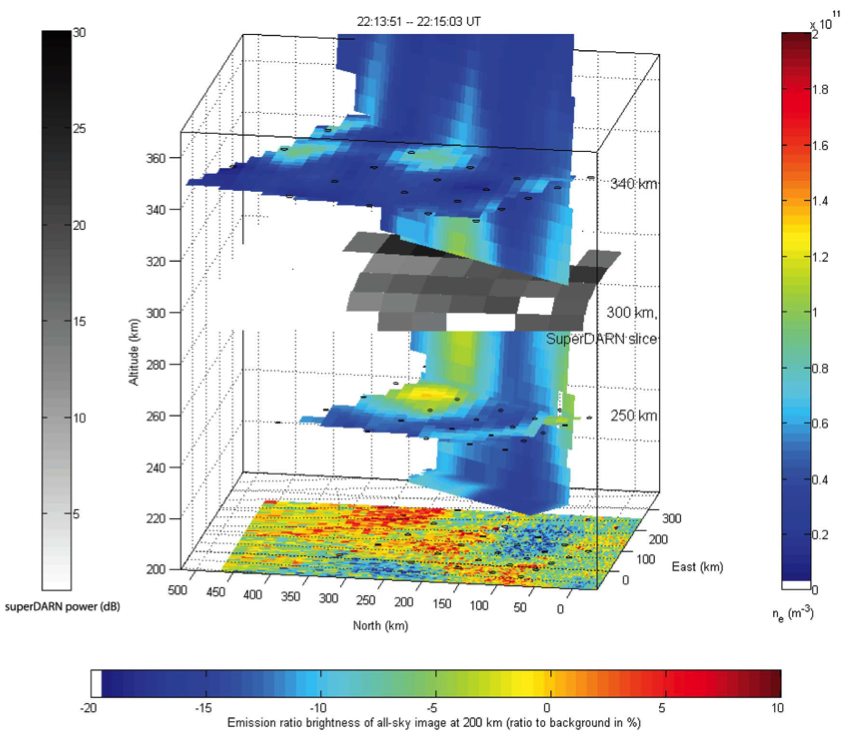
\includegraphics[width=4.0in]{patches}
% where an .eps filename suffix will be assumed under latex, 
% and a .pdf suffix will be assumed for pdflatex; or what has been declared
% via \DeclareGraphicsExtensions.
\caption{Example of polar cap patches seen in RISR and SuperDARN, from \cite{Dahlgren:2012dq}}
\label{fig:patches}
\end{figure}

Large horizontal gradients also occur during geomagnetic storms which can produce large flows.  This can create large disparities in Ion temperature as heating is occurring \cite{Zettergren:2008ba},\cite{semeter:plasmatransport2012}.  During these storms ion temperatures can go from 500$^\circ$ K to over 1500$^\circ$ K in the order of kilometers.

These high gradient events can cause some upridictible errors where two plasma population interface.  These errors can be quite complex due to the nonlinear nature of the inversion process\cite{Vallinkoski1990665}.  Similar behavior has been observed during times of auroral turbulence where shear flows seems to have caused non isotropic temperature measurements\cite{knudsen1993}. 
%\subsection*{Small Structure Events}
%\cite{semeter2010CI}

\subsubsection{High Speed Events}
At times the ionosphere can be come locally unstable this can create a number of different types of turbulent events. Langmuir turbulence can create coherent structures that will be detected by ISR systems \cite{akbari:2013lt}.  These structures change on the order of one pulse repetition interval of the radar.

%Resolving these high speed events are of great interest but also a challenge.  In ISR systems each pulse is used as a sample of a spectral averaging procedure.  It is assumed that these spectrums are identical independent samples.  If spectrum changes during this time, errors in the measurement could take place.  These errors are often unpredictable due to the nonlinear fitting used to fit the spectrum with the plasma parameters.
 %\cite{Dahlgren:2013ip}
%In the past researchers have studied errors associated with different plasma distributions mixing together.  These errors can be quite complex due to the nonlinear nature of the inversion process\cite{Vallinkoski1990665}.  Similar behavior has been observed during times of auroral turbulence where shear flows seems to have caused non isotropic temperature measurements\cite{knudsen1993}. 


\subsection{Inverse Problems}


\subsection{Outline of dissertation}
For this dissertation we will be proposing to improve the spatial and time sampling of the ISR systems.  New phased array radar systems have allowed for an unprecedented amount of flexibility in sampling the environment.  As such there has been no optimal way developed as of yet to sample this space.  Currently ISR systems integrate their spectral estimate in time only.  In order to get a statistical desirability of their measurements these systems may have to integrate for a long period of time.  It may be possible to integrate across different beams if stationarity can be found.  Other techniques could also be investigated such as well to try to improve the ISR measurements.

\section{Contributions}
Specific contributions of this research are summarized below.

\begin{enumerate}
\item Development of a theoretical framework for the forward model of 3-D ISR plasma parameter reconstructions.
\item Creating a framework full simulation of an ISR system that can which yield synthetic complex voltages.
\item A software package, named STISRS (Space-Time ISR Simulator), has be derived from previously mentioned simulation framework has been made available to other researchers.
\item A detailed analysis of the simulation framework using STISRS.
\item A new method for inverting the forward model 3-D ISR plasma parameter reconstructions.
\end{enumerate}